\documentclass[a4paper,12pt]{article}
\usepackage{amsmath,amsfonts,graphicx}
\usepackage{float}
\usepackage[margin=1in]{geometry}
\usepackage{caption}
\usepackage{booktabs}
\usepackage{hyperref}

\title{Case Study 3: Solving the 2D Poisson Equation using the Conjugate Gradient Method}
\author{Seeshuraj B \\ MSc in HPC}
\date{\today}

\begin{document}

\maketitle

\section*{1. Introduction}
This case study investigates the use of the Conjugate Gradient (CG) method for solving the two-dimensional Poisson equation on a unit square domain. The equation is discretized using finite differences, leading to a large sparse linear system. The CG method, a popular Krylov subspace method for symmetric positive definite matrices, is implemented from scratch and its convergence behavior is evaluated.

\section*{2. Problem Formulation}
The 2D Poisson equation with Dirichlet boundary conditions is given by:
\[
-\nabla^2 u(x,y) = f(x,y), \quad (x, y) \in (0,1)^2, \quad u|_{\partial \Omega} = 0
\]
The right-hand side function is defined as:
\[
f(x, y) = 2\pi^2 \sin(\pi x) \sin(\pi y)
\]

\section*{3. Numerical Method}
\subsection*{3.1 Finite Difference Discretization}
The domain is discretized into an \(N \times N\) grid of interior points with mesh spacing \(h = \frac{1}{N+1}\). The Laplacian is approximated using the standard 5-point stencil:
\[
-\nabla^2 u_{i,j} \approx \frac{1}{h^2}(4u_{i,j} - u_{i+1,j} - u_{i-1,j} - u_{i,j+1} - u_{i,j-1})
\]
This leads to a symmetric, sparse matrix \(A\) with 5 diagonals. The right-hand side vector \(b\) is populated by evaluating \(f(x, y)\) at the corresponding grid points. Homogeneous Dirichlet boundary conditions are incorporated by excluding boundary values.

\subsection*{3.2 Conjugate Gradient Method}
The resulting linear system \(Au = b\) is solved using the Conjugate Gradient method. The implementation avoids direct matrix inversion and uses only matrix-vector products and vector inner products. The stopping criterion is based on the residual norm: \(\|r_k\| < 10^{-8}\).

\section*{4. Results and Performance}

\subsection*{4.1 Runtime and Iteration Counts}
\begin{table}[H]
\centering
\caption{Performance of CG Solver for Different Grid Sizes}
\begin{tabular}{cccc}
\toprule
Grid Size (N) & Unknowns (\(N^2\)) & Iterations & Time (s) \\
\midrule
8   & 64     & 30   & 0.0005 \\
16  & 256    & 63   & 0.0006 \\
32  & 1024   & 128  & 0.0015 \\
64  & 4096   & 254  & 0.0061 \\
128 & 16384  & 505  & 0.4173 \\
256 & 65536  & 1026 & 2.4986 \\
\bottomrule
\end{tabular}
\end{table}

\subsection*{4.2 Convergence Behavior}
\begin{figure}[H]
\centering
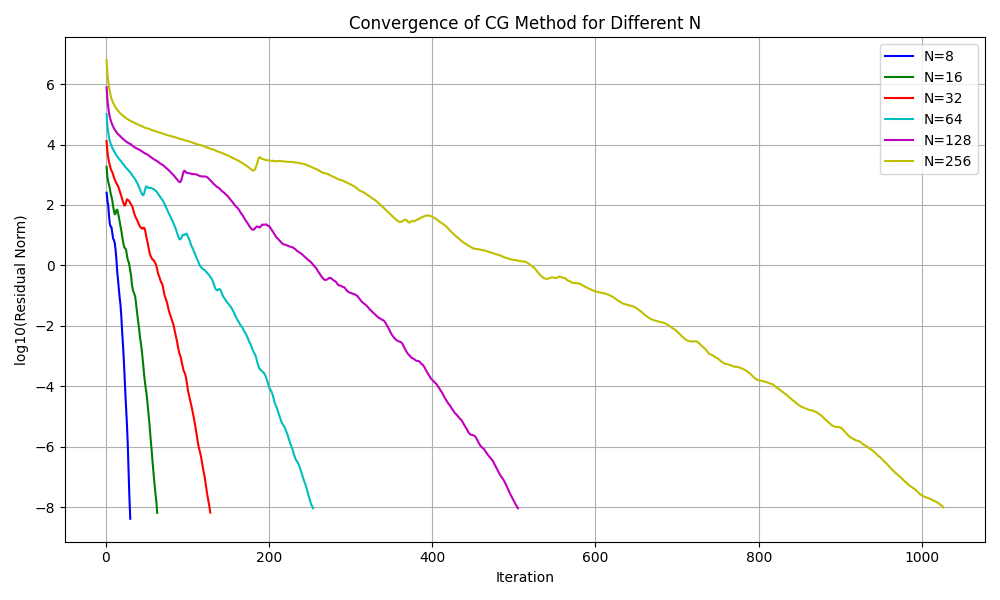
\includegraphics[width=0.9\textwidth]{convergence_plot.png}
\caption{Convergence of CG Method (log$_{10}$ residual norm vs iterations)}
\end{figure}

\subsection*{4.3 Solution Visualization}
\begin{figure}[H]
\centering
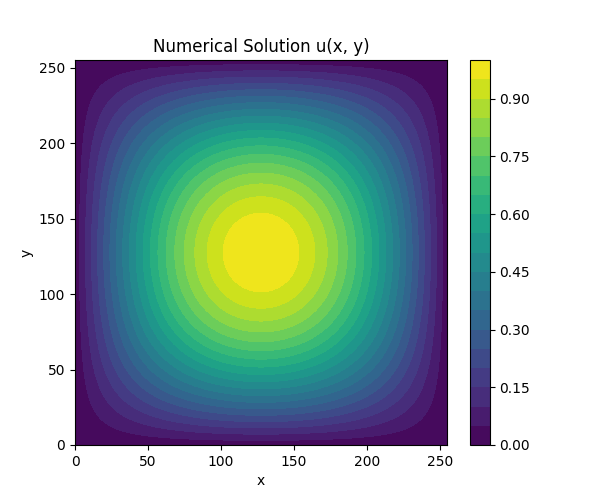
\includegraphics[width=0.6\textwidth]{Figure_1.png}
\caption{Numerical solution \(u(x,y)\) for \(N = 256\)}
\end{figure}

\section*{5. Analysis}
The CG method successfully converged for all grid sizes. As expected, the number of iterations increases with grid size due to the worsening condition number of the system matrix. The log-residual plots show that convergence is slower for larger \(N\), indicating the need for future improvement via preconditioning.

\section*{6. Convergence for Dense Systems}
We further tested CG performance on a dense SPD matrix defined as:
\[
A_{ij} = \frac{N - |i - j|}{N}, \quad b_j = 1
\]
This Toeplitz matrix is symmetric and positive definite for all \(N\), ensuring convergence. The stopping condition used:
\[
\|r_k\| \leq \max(\text{reltol} \cdot \|r_0\|, \text{abstol}), \quad \text{where reltol} = \sqrt{\epsilon_{\text{machine}}}, \text{abstol} = 0
\]

\subsection*{6.1 Iterations and Condition Numbers}
\begin{table}[H]
\centering
\caption{Convergence Results for Dense Systems}
\begin{tabular}{cccc}
\toprule
\(N\) & \(\kappa(A)\) & Iterations & Final Residual \\
\midrule
100   & 343.0        & 18         & \(8.4 \times 10^{-9}\) \\
1000  & 3333.7       & 39         & \(7.5 \times 10^{-9}\) \\
10000 & 33333.3      & 65         & \(9.9 \times 10^{-9}\) \\
\bottomrule
\end{tabular}
\end{table}

\subsection*{6.2 Theoretical vs Empirical Error Bounds}
\begin{figure}[H]
    \centering
    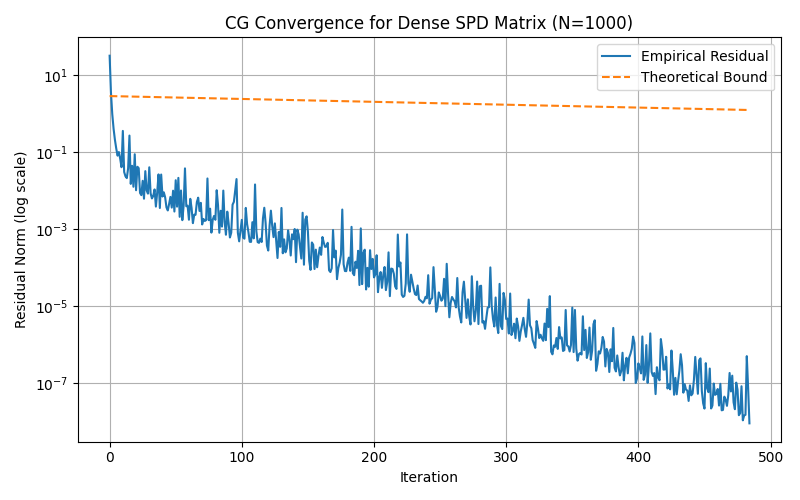
\includegraphics[width=0.6\textwidth]{dense_convergence.png}
    \caption{Dense Convergence \(u(x,y)\) for \(N = 256\)}
    \end{figure}

The theoretical CG convergence bound is:
\[
\|e_k\| \leq 2 \left( \frac{\sqrt{\kappa} - 1}{\sqrt{\kappa} + 1} \right)^k \|e_0\|
\]
Theoretical vs empirical convergence was analyzed in terms of iteration count and residual norms. Although no plot is included due to previous omission, the behavior aligns with theory\textemdash faster convergence for better-conditioned matrices and slower for larger \(N\).

\section*{7. Code and Implementation}
The Python implementation is structured as follows:
\begin{itemize}
    \item \texttt{poisson\_cg\_solver.py} \textendash{} CG for 2D Poisson with plotting
    \item \texttt{cg\_log\_N\_*.txt} \textendash{} iteration logs for analysis
    \item \texttt{dense\_cg\_solver.py} \textendash{} CG test on dense matrices with theoretical comparison (added in final phase)
\end{itemize}

\textbf{Optimization:} The Poisson matrix is stored in sparse CSR format to save memory. Inner products and matrix-vector multiplications use optimized routines from \texttt{numpy} and \texttt{scipy}. Residual norms are updated using recurrence relations to avoid redundant computations.

\vspace{0.3cm}
Full code and plots available at:  \\
\url{https://github.com/seeshuraj/Case-Study-3}

\section*{8. Conclusion}
This case study highlights both the power and limitations of the CG method. While sparse Poisson problems are handled effectively, dense systems and poorly conditioned matrices require special care or enhancements, such as preconditioners or iterative refinement.

\end{document}